\documentclass[oneside]{utmthesis}
%By default, print on two-side, can change to oneside printing 
%According to the new manual, should not mixed single-side with two-side printing

\usepackage{graphicx}
\usepackage{url} 
%\usepackage[pages=some]{background}
%\usepackage{lipsum}
\usepackage{pdflscape}

%%% You MUST load the natbib package if you want to use author-date bibliography style. Also remember to change the bibliography style at the bottom of the .tex file.
% Comment natbib for citation by number
%\usepackage{natbib}
%\let\cite\citep

%This is to make sure vertical spacing non-stretchable
\raggedbottom

\begin{document}

% Required information
\title{The Thesis Title}
\titletwo{Second Line (Optional)}
\titlethree{Third Line (Optional)}
\titlefour{Fourth Line (Optional)}
\author{The Author}
\degree{Bachelor of Science}
\specialization{Physics}
\intakeyear{2011}
\school{School of Electrical Engineering}
\faculty{Faculty of Engineering}
\titledate{October 2018}
\award{1}
% Options for Award 
% 1. Bachelor Degree Project Report
% 2. Master's Project Report (By course work)
% 3. Master's Dissertation (By course work and research)
% 4. Master's Thesis (By research)
% 5. Doctor of Philosophy Thesis
% 6. Other PhD Thesis
% 7. Generic PhD Thesis
% 8. Thesis Proposal
\superone{M.Y. Supervisor}
\supertwo{M.Y. Other Supervisor}
\superthree{M.Y. Superlong named supervisor}
% \superfour{Fourth SV}
% \superfive{Fifth SV}

% Mandatory pages
\coverpage
\superpage
\certification
\frontmatter
\maketitle
\declaration


\begin{dedication}
This thesis is dedicated to my father, who taught me that the best kind of knowledge to have is that which is learned for its own sake. It is also dedicated to my mother, who taught me that even the largest task can be accomplished if it is done one step at a time.\
\end{dedication}

\begin{acknowledgement}
Acknowledgement
\end{acknowledgement}


\begin{abstract}
A 1-page abstract is a \emph{movie (thesis) trailer}. Avoid summarizing
your Introduction chapter. Focus on the problem statement, hypothesis/objective,
research approach, quantitative validation summary, and implication
of your findings. For Ph.D., emphasize on original contributions.
\end{abstract}

\begin{abstrak}
The Malay abstract is written as the sentence structure of the English
abstract. All specific terms must be checked with Dewan Bahasa and
Pustaka (\url{http://prpm.dbp.gov.my/}). 
\end{abstrak}


\tableofcontents
\listoftables
\listoffigures


%List of abbreviation 
\listofabbre
\addabbre{ANN}{Artificial Neural Network}
\addabbre{PC}{Personal Computer}
\addabbre{SVM}{Support Vector Machine}
\addabbre{UTM}{Universiti Teknologi Malaysia}
\addabbre{XML}{Extensible Markup Language}


%List of symbols 
\listofsymbols
\addsymbol{$\gamma$}{Whatever}
\addsymbol{$\sigma$}{Whatever}
\addsymbol{$\varepsilon$}{Whatever}


%Uncomment if have appendices
\listofappendices


\mainmatter


\chapter{Introduction}

This template conforms with the Universiti Teknologi Malaysia 2018 new requirement \cite{utm:thesis:manual}.
Students who wish to learn more on LyX should refer to documentations
available here \cite{lyx:download}. You do not need to know deep
on LaTeX \cite{latex:wikibook} to use this LyX template.

\section{Definition of thesis }

\noindent \emph{Thesis} (generic term, see also Figure~\ref{fig1})
is a documented evidence of defined scope and length that a candidate
is 
\begin{itemize}
\item Understand relevant theoretical issues
\item Technically competent
\item Has critical-thinking ability
\item Able to \emph{conduct scholarly research}
\end{itemize}
\begin{figure}[h]
\begin{centering}

\includegraphics[width=1\textwidth]{./figs/pasted13}
\par\end{centering}
\caption{As it goes}
\label{fig1}

\end{figure}

Students have to write a scientific document of a defined scope and
length to demonstrate the achievement. According to UTM nomenclature
\begin{itemize}
\item UG FYP - \emph{report}
\item Master by taughtcourse project - \emph{project report}
\item Master by taughtcourse and research (mixed-mode) - \emph{dissertation}
\item Master by research and PhD - \emph{thesis}
\end{itemize}
Different degree level has different expectation
\begin{itemize}
\item Undergraduate report demonstrates the capacity to apply basic research
skills in an area of interest. At this level, the focus is on gaining
\textbf{broad competencies}. 
\item Masters thesis/dissertation/report demonstrates the capacity to apply
advanced research skills (i.e. move \textbf{beyond basic} research
skills) in an area of interest to a Master student is able to incorporate
some critical insights in his/her study. At this level, the focus
is on developing critical thinking in a subject area.
\item PhD thesis demonstrates the capacity to apply \textbf{specialized}
research skills (i.e. expert knowledge of a particular concept or
method) in an area of interest so that a PhD student can make significant
and original contribution to knowledge. At this level, the focus is
on identifying a 'gap' in knowledge and addressing it, hence advancement
in knowledge in a field of study.
\end{itemize}

\section{Main steps in thesis/dissertation/report writing}
\begin{itemize}
\item Plan/elaborate the outline
\begin{itemize}
\item A \emph{plot} for your thesis writing
\item Target: \emph{logical story} for the document
\item Results
\begin{itemize}
\item Stand-alone tables/graphs
\item Describe each, then number crunch
\item Use Appendices for detailed items
\end{itemize}
\end{itemize}
\item Get feedback from the supervisor
\item If you are writing in a language other than your mother language,
consider getting specialized editing help
\end{itemize}
\begin{figure}[h]
\begin{centering}
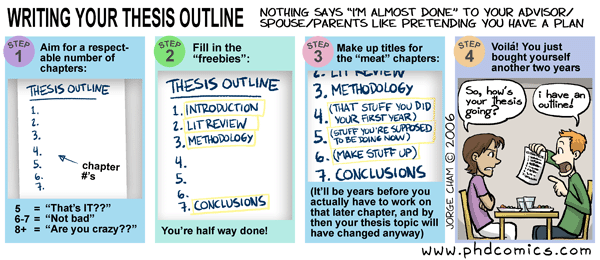
\includegraphics[width=0.8\textwidth]{./figs/pasted3}
\par\end{centering}
\caption{Thesis outline}

\end{figure}


\chapter{Thesis structure shown as a very very very very very very very very
very very very very very very very very very very very very very very
very long title}

\section{Thesis title (SPS guidelines)}
\begin{itemize}
\item Thesis title should be a concise description of the main focus and
contribution of the research. It should not contain more than 15 words
excluding grammatical words such as articles, conjunction and prepositions.
\item To avoid redundancy, titles should not contain phrases which reflect
research exercise such as \textquotedblleft An investigation of ...\textquotedblright ,
\textquotedblleft A preliminary study of ...\textquotedblright , \textquotedblleft A
study of ...\textquotedblright , \textquotedblleft Analysis of ...\textquotedblright ,
\textquotedblleft On the ...\textquotedblright , \textquotedblleft Theory
of ...\textquotedblright , \textquotedblleft Some ,,,\textquotedblright ,
and \textquotedblleft Toward a ...\textquotedblright .
\item Thesis title should not contain formulas, symbols or subscripts, Greek
letters, or other non-alphabetical symbols. Word substitutes should
be used instead. 
\item Thesis title should not contain acronyms or even acronyms in brackets
unless the term is commonly used in the field of the study (eg: DNA,
GPS). For example, \textquotedblleft GIS\textquotedblright{} should
be written as \textquotedblleft Geographical Information System\textquotedblright{}
and should not be written as \textquotedblleft Geographical Information
System (GIS)\textquotedblright .
\item Thesis title should not contain punctuation such as colon \textquotedblleft :\textquotedblright ,
semicolon \textquotedblleft ;\textquotedblright , etc. except commas
\textquotedblleft ,\textquotedblright{} when necessary.
\end{itemize}

\section{Flow of arguments }

Each thesis is unique and depends on the writer and the editor (your
supervisor). There is no cast-on-stone and rigid thesis structure.
The following example a good starting point:

\subsection{Thesis }

Thesis title should be a concise description of the main focus and
contribution of the research

\subsection{Abstract }
\begin{itemize}
\item A short summary of the the thesis/dissertation/report
\begin{itemize}
\item Describe the problem and the research approach
\item Emphasize the original contributions
\item A movie trailer and not a summary of thesis
\end{itemize}
\end{itemize}

\subsection{Introducing your work}
\begin{itemize}
\item An overview of the problem
\begin{itemize}
\item Problem motivation and why it is important
\item Problem definition highlight what had been done before and the research
gap to be studied, worthy a (PhD, Master, or UG) degree
\item Your hypothesis or objective of the thesis
\item Organization of the thesis -- you should guide the readers on what
to expect next
\end{itemize}
\item Make it readable by anyone
\end{itemize}

\subsection{Discussion of the problem and state-of-the-art solutions to problem }
\begin{itemize}
\item Usually titled as Literature Review
\item Not a literature survey in general, but rather a synthesis of the
state-of-the-art related to the thesis!
\begin{itemize}
\item Can also include a background information -- brief synthesis of the
most relevant aspects related to the thesis in order to help the reader
understand the context and the contributions coming from other disciplines.
\item It can also be used to better motivate the research question.
\item Identify gaps/limitations of existing state-of-the-arts
\item Background \& related work may overlap
\begin{itemize}
\item Need to discuss related work at start to set the scene
\item Need to discuss related work at end to demonstrate your originality
\item But not cut and paste!
\item Exercise your synthesis and critic skills!
\end{itemize}
\item Make the definitions precise, concise, and unambiguous. 
\end{itemize}
\end{itemize}

\subsection{Your proposed work}
\begin{itemize}
\item Usually entitled Methodology, but not necessary
\item Here you develop your conceptual contribution, i.e. the central concept
of your work
\begin{itemize}
\item Discussion of the thesis and different perspectives of analysis of
the research question
\begin{itemize}
\item Definition of problem
\item Formulation of concepts, definitions, theories
\end{itemize}
\item Research design
\begin{itemize}
\item Elaboration of frameworks, models, architectures
\item Methods and procedure, variables
\item May include description of a prototype system implementation and its
use towards solving the research problem 
\item Can include some context information (e.g. development software, test
environment, procedure, limitations, assumptions, range of validity)
\item But not too many details!!!
\end{itemize}
\end{itemize}
\end{itemize}

\subsection{Validation of hypothesis}
\begin{itemize}
\item Usually titled as Result and Discussion
\item Describe experiment details that provide evidence in support of your
thesis
\begin{itemize}
\item Developing a prototype may not enough to validate the thesis -- at
most it is a proof of feasibility of your system
\item Validation is about collecting (enough) evidence to convince the other
researchers about the validity of the thesis through
\begin{itemize}
\item A proper (systematic) method
\item Organized argumentation (is important)
\end{itemize}
\item Analysis and concepts form the heart of the work
\item It must state what was learned, not only the facts that were gathered! 
\end{itemize}
\end{itemize}

\subsection{Take home message to readers}
\begin{itemize}
\item Summarize what was learned and how it can be applied 
\begin{itemize}
\item Include the broader implications of your results
\item Do not repeat word for word the abstract, introduction or discussion
\item Mention the possibilities for future research
\end{itemize}
\end{itemize}

\subsection{References to back up your statements}
\begin{itemize}
\item If you make a statement, back it up with your own data or a reference
\begin{itemize}
\item All references cited in the text must be listed
\item UTM supports either the numbering or author-year format
\item Try to avoid inclusion of references as footnotes
\end{itemize}
\end{itemize}

\subsection{Appendices}
\begin{itemize}
\item This is an optional part
\begin{itemize}
\item It can include:
\begin{itemize}
\item Implementation details
\item Detailed experiment data
\end{itemize}
\item May be important to
\begin{itemize}
\item Convince the reader
\item Help others replicating the experiment
\end{itemize}
\item ... but are \textquotedblleft boring\textquotedblright{} or too detailed
to include in the main body of the thesis
\end{itemize}
\end{itemize}

\section{Suggested order for writing}
\begin{itemize}
\item Begin by writing the chapters that describe your research (2,3, 4,
and 5 in the above outline)
\item Define all technical terms and make the definitions precise and formal
\item After reading the main chapters to verify terminology, write the conclusions
\item Write the introduction
\item Complete with an abstract
\end{itemize}

\section{The revision journey }
\begin{itemize}
\item Revise them and start getting feedback 
\begin{itemize}
\item \textbf{think-plan-write-revise} cycles
\end{itemize}
\item Get early feedback from colleagues
\begin{itemize}
\item Starting with the key chapters
\end{itemize}
\item Carefully revise those chapters before giving them to your supervisor
\item When you have a complete draft 
\begin{itemize}
\item Consider 2 or 3 complete revision/editing iterations!
\item Could be more
\end{itemize}
\end{itemize}

\chapter{Results and Discussion}

\section{Graphic and Images}
A good thesis needs good diagrams/graphs/illustrations. Spend some
time doing in properly. A good picture tells a thousand words.

\section{Floats}
\begin{itemize}
\item A float doesn't have a fixed location. 
\begin{itemize}
\item It can ``float'' forward or backward to wherever it fits best to
get a high quality layout. 
\item Caption as part of a float.
\end{itemize}
\item Float Placement
\begin{itemize}
\item [h]: try to place the float at the
position where it is inserted 
\item [t]: try to place the float at the top
of the current page
\item [b]: try to place the float at the
bottom of the current page
\item [p]: try to place the float at an own
page 
\end{itemize}
\end{itemize}

\begin{figure}[!ht]
	\centering
	
\includegraphics[width=0.5\linewidth]{./figs/utm02}
	\caption{Example of a figure. This is a long, very long, long long, long caption.  You can give a shorter caption for the ``list of figures" using the square bracket symbol.}
\end{figure}


\begin{table}[!ht]
\centering
\caption{The role of statistical quality engineering tools and methodologies}
\vspace{\baselineskip}
\begin{tabular}{l c c}
  \hline
  \hline
  Temperature & Resonant Frequency & Q factor\\
  \hline
  13 mK $\pm$ 1 mK & 16.93 & 811 \\
  40 mK $\pm$ 1 mK & 16.93 & 817 \\
  100 mK $\pm$ 1 mK & 16.93 & 815 \\
  300 mK $\pm$ 1 mK & 16.93 & 806\\
  500 mK $\pm$ 1 mK & 16.93 & 811\\
  800 mK $\pm$ 5 mK & 16.93 & 814\\
  1000 mK $\pm$ 5 mK & 16.93 & 806 \\
  \hline
  \hline
\end{tabular}
\end{table}

\begin{landscape}
\begin{table}[p]
\centering
\caption{The role of statistical quality engineering tools and methodologies}
\vspace{\baselineskip}
\begin{tabular}{l c c}
  \hline
  \hline
  Temperature & Resonant Frequency & Q factor\\
  \hline
  13 mK $\pm$ 1 mK & 16.93 & 811 \\
  40 mK $\pm$ 1 mK & 16.93 & 817 \\
  100 mK $\pm$ 1 mK & 16.93 & 815 \\
  300 mK $\pm$ 1 mK & 16.93 & 806\\
  500 mK $\pm$ 1 mK & 16.93 & 811\\
  800 mK $\pm$ 5 mK & 16.93 & 814\\
  1000 mK $\pm$ 5 mK & 16.93 & 806 \\
  \hline
  \hline
\end{tabular}
\end{table}
\end{landscape}


\chapter{Conclusion}
\section{Research Outcomes}
\section{Contributions to Knowledge}
\section{Future Works}

%select one
%Use authordate with natbib, comment if using numbering
%\bibliographystyle{utmthesis-authordate}
%When using numbering, comment when using author-year
%Numbering does not use \citep nor citet (natbib)
\bibliographystyle{utmthesis-numbering}
\bibliography{reference}

%-----------List of Publication-----------%
%This is not required for FYP project report
\listofpublications

\noindent \textbf{Journal with Impact Factor}
\begin{enumerate}
\item Paper 1
\item Paper 2
\end{enumerate}
\textbf{Indexed Journal (SCOPUS)}
\begin{enumerate}
\item Paper 3
\end{enumerate}
\noindent \textbf{Non-Indexed Journal}
\begin{enumerate}
\item Paper 4
\end{enumerate}
\noindent \textbf{Indexed conference proceedings}
\begin{enumerate}
\item Paper 5
\end{enumerate}
\noindent \textbf{Non-Indexed conference proceedings}
\begin{enumerate}
\item Paper 6
\end{enumerate}


\appendix
\chapter{Time-series Data}
Some data

%This is required to make List of Appendices possible. Remove when have no appendix.
\endmatter
\end{document}
